\documentclass[../../Main_ManuscritThese.tex]{subfiles}

\subfileGlobal{
\renewcommand{\RootDir}[1]{./Text/Annexes/#1}
}

% For cross referencing
% \subfileLocal{
% \externaldocument{../../Text/Introduction/build/Introduction}
% \externaldocument{../../Text/Chapter2/build/Chapter2}
% \externaldocument{../../Text/Chapter3/build/Chapter3}
% \externaldocument{../../Text/Chapter4/build/Chapter4}
% \externaldocument{../../Text/Chapter5/build/Chapter5}
% \externaldocument{../../Text/Conclusion/build/Conclusion}
% }

%%%%%%%%%%%%%%%%%%%%%%%%%%%%%%%%%%%%%%
%% CHAPTER TITLE
%%%%%%%%%%%%%%%%%%%%%%%%%%%%%%%%%%%%%%

\begin{document}
%	


\begingroup

%% Le chapitre est numéroté A
% \setcounter{chapter}{0}
% \renewcommand{\thechapter}{\Alph{chapter}}%
\appendix
\setcounter{chapter}{5}
\renewcommand{\thechapter}{A}
%% Le titre doit être entre les traits de la 1ere page du chapitre
\TitleBtwLines
\chapter{Appendix}


\label{chap:appendix}
\pagestyle{appendixStyle}
\minitoc
% \section{Likelihood ratio test for misspecified nested models}
% This section follows the proofs of~\cite{white_maximum_1982}. The observations $Y$ are following the law
% with true density $p_Y$, and $n$ samples are available $y=\{y_i\}$.
% We have a family of distributions $\{p_{Y\mid \KK}\}$.  The quasi
% log-likelihood is
%   \begin{equation}
%     \mathcal{L}(\kk; y) = \frac{1}{n}\sum_{i=1}^{n} \log p_{Y \mid \KK}(y;\kk)
%   \end{equation}

%   \begin{align}
%     A_n(\kk) = \frac{1}{n} \sum_{i=0}^n \frac{\partial^2 \log p_{Y \mid \KK}(y\mid\kk)}{\partial \kk_i \partial \kk_j} \\
%     B_n(\kk) = \frac{1}{n} \sum_{i=0}^n \pfrac{p_{Y\mid \KK}(y \mid \kk)}{\kk_i} \pfrac{p_{Y\mid \KK}(y \mid \kk)}{\kk_j}
%   \end{align}

%   \begin{align}
%     A(\kk) &= \Ex\left[\frac{\partial^2 \log p_{Y\mid \KK}(y \mid \kk)}{\partial \kk^2}\right]\\
%     B(\kk) &= \Ex\left[\pfrac{\log p_{Y\mid \KK}(y \mid \kk)}{\kk}\pfrac{\log p_{Y\mid \KK}(y \mid \kk)}{\kk}^T\right]
%   \end{align}

%   If the model is well-specified, in other words if there exists $\kk_0$ such that $p_Y = p_{Y\mid \KK}(\cdot \mid\kk_0)$, $A(\kk) = -B(\kk)$:
%   \begin{align}
%     \frac{\partial^2 \log p_{Y\mid \KK}(y \mid \kk)}{\partial \kk^2} &= \pfrac{}{\kk}\left(\frac{1}{p}\pfrac{p}{\kk}\right) \\
%     &= \frac{1}{p}\frac{\partial^2 p}{\partial \kk^2} - \frac{1}{p^2}\left(\pfrac{p}{\kk}\right)^2 = \frac{1}{p}\frac{\partial^2 p}{\partial \kk^2} - \left(\pfrac{\log p}{\kk}\right)^2
%   \end{align}
%   Taking the expectation, we have
%   \begin{align}
%     A(\kk) &= \Ex\left[\frac{\partial^2 \log p_{Y\mid \KK}(y \mid \kk)}{\partial \kk^2}\right] \\
%            &= -\Ex\left[\left(\pfrac{\log p}{\kk}\right)^2\right] + \Ex\left[\frac{1}{p}\frac{\partial^2 p}{\partial \kk^2}\right]
%   \end{align}
%   and the last term is
%   \begin{align}
%      \Ex\left[\frac{1}{p}\frac{\partial^2 p}{\partial \kk^2}\right] = \int_{\Yspace} \frac{1}{p}\frac{\partial^2 p}{\partial \kk^2} p_{Y}(y) \,\mathrm{d}y
%   \end{align}
%   If the inverse exist,
%   then
%   \begin{align}
%     C_n(\kk) &= A_n(\kk)^{-1} B_n(\kk) A_n(\kk) \\
%     C(\kk) &= A(\kk)^{-1}B(\kk)A(\kk)
%   \end{align}

  \section{Lognormal approximation of the ratio of normal random variables}
  \label{sec:lognorm_ratio}
  Let $X$ and $Y$ be two correlated normal random variables:
  \begin{align}
    X &\sim \mathcal{N}(\mu_X, \sigma^2_X) \\
    Y &\sim \mathcal{N}(\mu_Y, \sigma^2_Y) \\
    \rho &= \frac{\Cov[X,Y]}{\sigma_X \sigma_Y} \\
    \begin{bmatrix}
      X \\ Y
    \end{bmatrix} &\sim \mathcal{N}\left(%
    \begin{bmatrix}
      \mu_X \\ \mu_Y
    \end{bmatrix};%
    \begin{bmatrix}
      \sigma^2_X  & \rho \sigma_X \sigma_Y \\
      \rho\sigma_X \sigma_Y & \sigma^2_Y
    \end{bmatrix} \right)
  \end{align}
  Let us assume that both random variable are positive with high probability, then the ratio $T=X/Y$ is defined and positive with high probability. We will first rewrite $T$ using the centered random variables $X_0=X-\mu_X$ and $Y_0 = Y-\mu_Y$:
  \begin{equation}
    T = \frac{\mu_X}{\mu_Y}\frac{1 + \frac{X_0}{\mu_X}}{1 + \frac{Y_0}{\mu_Y}}
  \end{equation}
  and we can then take its logarithm
  \begin{equation}
    \log T = \log\left(\frac{\mu_X}{\mu_Y}\right) + \log\left(1 + \frac{X_0}{\mu_X}\right) -\log\left(1 + \frac{Y_0}{\mu_Y}\right)
  \end{equation}
  
  So if $X_0 / \mu_X$ and $Y_0/ \mu_Y$ are small, i.e.\ if $\mu_X \gg \sigma_X$ and $\mu_Y \gg \sigma_Y$, by Taylor's expansion of the $\log$, we have
  \begin{align}
    \log T & \approx \log\left(\frac{\mu_X}{\mu_Y}\right) + \frac{X_0}{\mu_X} - \frac{Y_0}{\mu_Y}
% \\
%     & \sim \mathcal{N}\left(\log\left(\frac{\mu_X}{\mu_Y}\right), \frac{\sigma_X^2}{\mu_X^2}+\frac{\sigma_Y^2}{\mu_Y^2}\right)
  \end{align}
  The joint distribution of $X_0$ and $Y_0$ is known:
  \begin{align}
    \begin{bmatrix}
      X - \mu_X \\ Y - \mu_Y
    \end{bmatrix} = 
    \begin{bmatrix}
      X_0 \\ Y_0
    \end{bmatrix} \sim \mathcal{N}\left(%
    \begin{bmatrix}
      0 \\ 0
    \end{bmatrix};%
    \begin{bmatrix}
      \sigma^2_X  & \rho \sigma_X \sigma_Y \\
      \rho\sigma_X \sigma_Y & \sigma^2_Y
    \end{bmatrix} \right)%
  \end{align}
  and by scaling by $1/\mu_X$ and $1/\mu_Y$, we have
  \begin{align}
    \begin{bmatrix}
      \frac{1}{\mu_X} & 0 \\
      0 & \frac{1}{\mu_Y}
    \end{bmatrix}
    \begin{bmatrix}
      X_0 \\ Y_0
    \end{bmatrix}=
    \begin{bmatrix}
      X_0/\mu_X \\ Y_0/ \mu_Y
    \end{bmatrix} \sim \mathcal{N}\left(%
    \begin{bmatrix}
      0 \\ 0
    \end{bmatrix};%
    \begin{bmatrix}
      \frac{\sigma^2_X}{\mu_X^2}  & \rho \frac{\sigma_X \sigma_Y}{\mu_X \mu_Y} \\
      \rho \frac{\sigma_X \sigma_Y}{\mu_X \mu_Y}& \frac{\sigma^2_Y}{\mu_Y^2}
    \end{bmatrix} \right)%
  \end{align}

  Thus
  \begin{equation}
    \frac{X_0}{\mu_X} - \frac{Y_0}{\mu_Y} \sim \mathcal{N}\left(0;\frac{\sigma^2_X}{\mu_X^2} + \frac{\sigma^2_Y}{\mu_Y^2} - 2 \rho \frac{\sigma_X \sigma_Y}{\mu_X \mu_Y} \right)
  \end{equation}
  
  A first approximation is then to consider the ratio to be log-normally distributed, and
  \begin{equation}
    \log T \sim \mathcal{N}\left(\log \frac{\mu_X}{\mu_Y}; \frac{\sigma^2_X}{\mu_X^2} + \frac{\sigma^2_Y}{\mu_Y^2} - 2 \rho \frac{\sigma_X \sigma_Y}{\mu_X \mu_Y} \right)
  \end{equation}
  
  % \begin{align}
  %   \Ex[T] &= \exp\left(\log\left(\frac{\mu_X}{\mu_Y}\right) + \frac{1}{2}\left(\frac{\sigma_X^2}{\mu_X^2}+\frac{\sigma_Y^2}{\mu_Y^2} \right)\right)\\
  %          &=\left(\frac{\mu_X}{\mu_Y}\right) \exp\left(\frac{\sigma_X^2}{2\mu_X^2}+\frac{\sigma_Y^2}{2\mu_Y^2}\right) \\
  %   \Var[T] &= \left(\exp\left(\frac{\sigma_X^2}{\mu_X^2}+\frac{\sigma_Y^2}{\mu_Y^2}\right)-1 \right)\Ex[T]^2
  % \end{align}

%   \subsection{Transformation}
%   \cite{hayya_note_1975}
% \begin{align}
%   t =\frac{\mu_Y T - \mu_X}{\sqrt{\sigma^2_X - 2T\rho\sigma_Y\sigma_X + T^2\sigma_Y^2}} \sim \mathcal{N}(0, 1)
% \end{align}

% Conservative rule of thumb: if $\mu_Y/\sigma_Y \leq 0.09$ and $\mu_X / \sigma_X > 0.19$
\newpage
\section{Full sediment repartition in the Bay of Biscay and the English Channel}
 \label{sec:sediments_full}
\begin{figure}[ht]
  \centering
  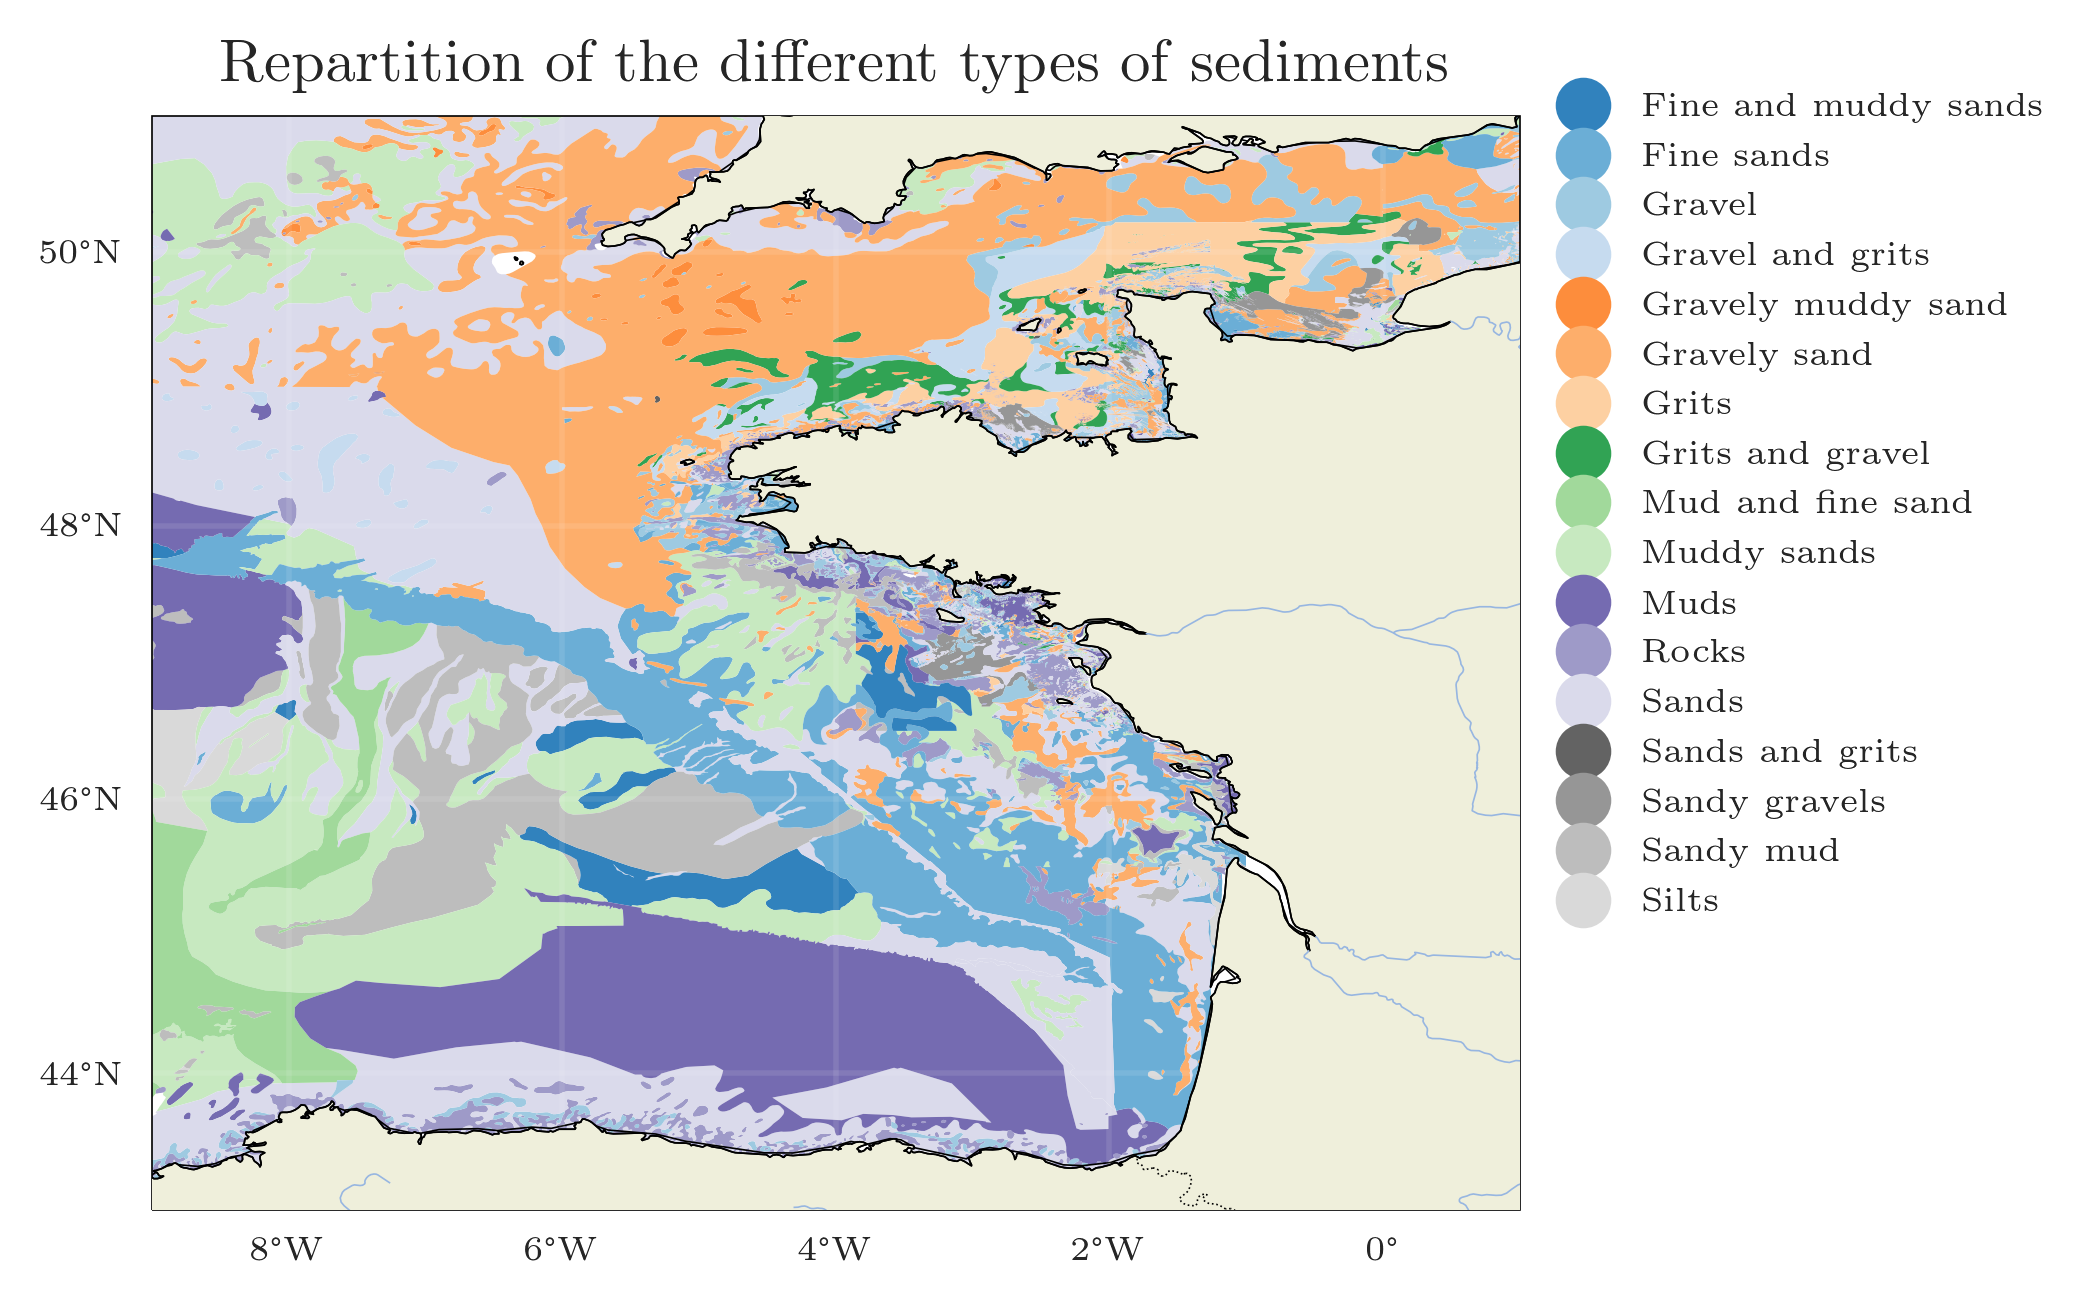
\includegraphics{/home/victor/acadwriting/Manuscrit/Text/Chapter5/img/sediments_full.png}
  \caption{\label{fig:sediments_full} Full sediments repartition}
\end{figure}
\clearpage
\section{Misspecified deterministic calibration}
\clearpage
\begin{figure}[ht]
  \centering
  \includegraphics[scale=1.]{/home/victor/optimisation_dahu/1b/map_log_400.png}
\end{figure}
\begin{figure}[ht]
  \centering
  \resizebox{1\textwidth}{!}{\input{/home/victor/optimisation_dahu/1b/ctrl_true.pgf}}
\end{figure}
% \begin{figure}[ht]
%   \centering
%   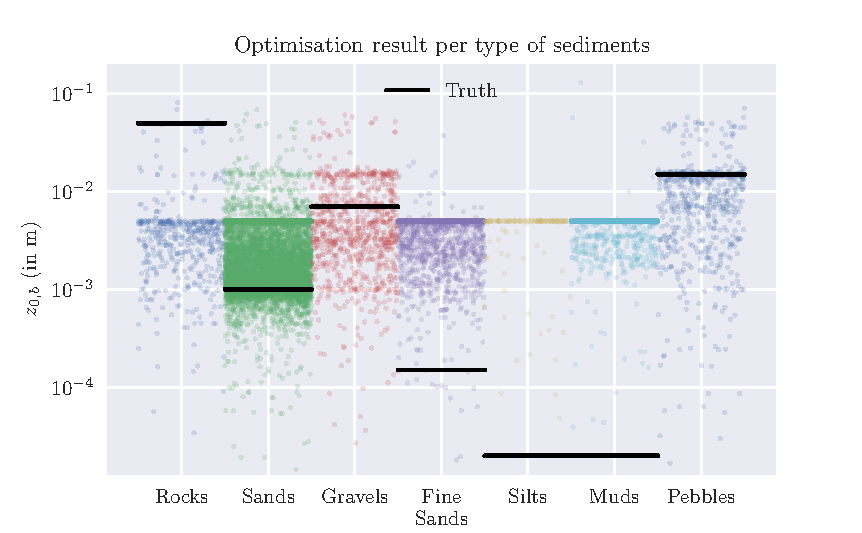
\includegraphics[scale=0.7]{/home/victor/optimisation_dahu/1b/optimisation_type_sediments.pdf}
% \end{figure}
\clearpage


\begin{figure}[ht]
  \centering
  \includegraphics{/home/victor/optimisation_dahu/2b/map_log_400.png}
\end{figure}
\begin{figure}[ht]
  \centering
    \resizebox{1\textwidth}{!}{\input{/home/victor/optimisation_dahu/2b/ctrl_true.pgf}}
\end{figure}
\clearpage
\begin{figure}[ht]
  \centering
  \includegraphics{/home/victor/optimisation_dahu/3/map_111.png}
\end{figure}
\begin{figure}[ht]
  \centering
  \includegraphics{/home/victor/optimisation_dahu/3/ctrl_plot.png}
\end{figure}
\clearpage
\begin{figure}[ht]
  \centering
  \includegraphics{/home/victor/optimisation_dahu/4/map_199.png}
\end{figure}
\begin{figure}[ht]
  \centering
  \includegraphics{/home/victor/optimisation_dahu/4/ctrl_plot.png}
\end{figure}
\clearpage
\begin{figure}[ht]
  \centering
  \includegraphics{/home/victor/optimisation_dahu/5/map_199.png}
\end{figure}
\begin{figure}[ht]
  \centering
  \includegraphics{/home/victor/optimisation_dahu/5/ctrl_plot.png}
\end{figure}
\clearpage
\begin{figure}[ht]
  \centering
  \includegraphics{/home/victor/optimisation_dahu/6/map_199.png}
\end{figure}
\begin{figure}[ht]
  \centering
  \includegraphics{/home/victor/optimisation_dahu/6/ctrl_plot.png}
\end{figure}
\clearpage
\begin{figure}[ht]
  \centering
  \includegraphics{/home/victor/optimisation_dahu/7/map_199.png}
\end{figure}
\begin{figure}[ht]
  \centering
  \includegraphics{/home/victor/optimisation_dahu/7/ctrl_plot.png}
\end{figure}
\clearpage
\begin{figure}[ht]
  \centering
  \includegraphics{/home/victor/optimisation_dahu/8/map_199.png}
\end{figure}
\begin{figure}[ht]
  \centering
  \includegraphics{/home/victor/optimisation_dahu/8/ctrl_plot.png}
\end{figure}
\clearpage
\begin{figure}[ht]
  \centering
  \includegraphics{/home/victor/optimisation_dahu/9/map_199.png}
\end{figure}
\begin{figure}[ht]
  \centering
  \includegraphics{/home/victor/optimisation_dahu/9/ctrl_plot.png}
\end{figure}
\clearpage




\pagestyle{appendixStyle}

%%%%%%%%%%%%%%%%%%%%%%%%%%%%%%%%%%%%%%%%%%%%%%%%%%%%%%%


%%%%%%%%%%%%%%%%%%%%%%%%%%%%%%%%%%%%%%
%% BIB
%%%%%%%%%%%%%%%%%%%%%%%%%%%%%%%%%%%%%%
\subfileLocal{
	\pagestyle{empty}
	\bibliographystyle{alpha}
	\bibliography{/home/victor/acadwriting/bibzotero}

}

\endgroup

\end{document}

%%% Local Variables:
%%% mode: latex
%%% TeX-master: "../../Main_ManuscritThese"
%%% End:
